\documentclass[onecolumn]{aastex63}
\usepackage{natbib}
%\definecolor{orcidlogocol}{HTML}{A6CE39}
\bibliographystyle{aasjournal}

\begin{document}

\title{PLANETESIMAL ACCRETION AT SHORT ORBITAL PERIODS}

\author{Spencer C. Wallace}
\affiliation{Astronomy Department, University of Washington, Seattle, WA 98195}


\author{Thomas R. Quinn}
\affiliation{Astronomy Department, University of Washington, Seattle, WA 98195}

\begin{abstract}
Abstract goes here
\end{abstract}

\section{Introduction} \label{sec:intro}

Intro text goes here \citep{Wallace2019}

\section{Collision and Relaxation Timescale}

The motivation for this project comes from the realization that the collision timescale and the relaxation time (which sets the timescales for things like viscous stirring and dynamical friction (cite ida 1993)) do not scale proportionately with orbital period. At sufficiently long orbital periods, the relaxation time is shorter than the collision time. This means that as planetesimals grow, the velocity distribution of bodies reacts to the changing mass distribution, which alters the growth mode. When this condition is met, oligarchic growth can commence (cite ki 1998), which keeps the planetary embryos on circular orbits and restricts their growth.

Because these two timescales scale differently with orbital period (or equivalently semimajor axis), they should eventually cross as one gets close enough to the host star. In regions where the collision timescale is shorter than the growth time, the embryos will maintain eccentric orbits as they grow, which greatly widens their feeding zones. Because they do not settle onto circular orbits, the timescale for orbital instability, which marks the beginning of the final planet-forming phase, should be much shorter.

\subsection{Collision Timescale}

The timescale for collisions is set by

\begin{equation}
	t_{coll} = \frac{1}{n \sigma v}
\end{equation}

\noindent where $n$ is the number density of planetesimals, $\sigma$ is the cross section for collisions and $v$ is the typical encounter velocity between planetesimals. 

The number density of planetesimals is set by

\begin{equation}
    n = \frac{\Sigma \Omega}{2 m v}
\end{equation}

\noindent where $\Sigma$ is the surface density of solids in the disk, $\Omega$ is the orbital frequency and $m$ is the mass of a planetesimal. For our purposes, we will assume that the surface density profile follows a power law such that $\Sigma = A r^{-\alpha}$. Planetesimals are typically large enough to exert a significant gravitational pull on each other, which enhances the collision cross section beyond its geometric value

\begin{equation}
	\sigma = \pi s^{2} \left( 1 + \frac{v_{esc}^{2}}{v^{2}} \right)
\end{equation}

\noindent where $s$ is the radius of a planetesimal and $v_{esc}$ is the escape velocity from the surface of a planetesimal. Finally, $v$ is given by (cite Lissauer 1993)

\begin{equation}
	v = \sqrt{\left<  e^{2} \right>^{1/2} + \left< i^{2} \right>^{1/2}} v_{k}
\end{equation}

\noindent For simplicity, we will assume that the rms eccentricity and inclination of the planetesimals does not vary with orbital distance. Putting this all together, the collision timescale scales with the orbital distance and the surface density profile parameters ($A$, $\alpha$) like

\begin{equation}
	t_{coll} \sim A^{-1} r^{\alpha + 1/2}
\end{equation}

Note that a surface density profile with $\alpha < -1$ produces a collision timescale that scales more steeply than the orbital timescale. In this case, an N-body simulation will get more computationally expensive with orbital distance because the time step size scales with the orbital timescale.

In terms of encounter velocity, gravitational focusing is the only thing that effects collision timescale. This is because number density of planetesimals $n$ scales with $v^{-1}$, which cancels with the other $v$ term. This leaves us with $t_{coll} \sim v^{2}$ or, in terms of the rms eccentricity (assuming the rms inclination is coupled to the eccentricity)

\begin{equation}
    t_{coll} \sim \left< e^{2} \right>^{1/2}
\end{equation}

\subsection{Relaxation Timescale}

The relaxation timescale is given by (citation)

\begin{equation}
    t_{relax} = \frac{v^3}{n \pi G^{2} m^{2} \ln \lambda}
\end{equation}

\noindent where $G$ is the gravitational constant and $\ln \lambda$ is the Coulomb logarithm. Using the same assumptions as above, the relaxation time scales with orbital distance and the surface density profile parameters as

\begin{equation}
    t_{relax} \sim A^{-1} r^{\alpha - 1/2}
\end{equation}

Note that this has a different dependence on $r$ than the collision timescale. Taking the ratio of these two timescales gives

\begin{equation}
    \frac{t_{relax}}{t_{coll}} \sim r^{-1}
\end{equation}

The relaxation time drops relative to the collision timescale with distance.

In terms of encounter velocity, the relaxation time scales as $t_{relax} \sim v^{4}$. Taking the ratio of the scaling for the collision and relaxation time with rms eccentricity gives (because there is a geometric term in the collision cross section, the ratio of these two timescales still goes as $v^{4}$)

\begin{equation}
    \frac{t_{relax}}{t_{coll}} \sim \left< e^{2} \right>
\end{equation}

Therefore, a dynamically hot disk will have a better chance of inhibiting oligarchic growth. All planetesimal disks will tend toward this state because gravitational stirring is most effective in a cold disk. So long as gas drag does not strongly damp things, this condition could be met. Why doesn't this happen for Kokubo + Ida simulations?

Figure \ref{fig:time_eq_gf} shows the Hill eccentricity required for these two timescales to be equal as a function of orbital period (solid lines). Regions above the curves represent parameter combinations in which the relaxation timescale is longer. This is assuming that the planetesimals have an internal bulk density of 2 g cm$^{-3}$ and their collision cross section is enhanced by a factor of $f_{pl}$ to make the computation faster.

\begin{figure}
    \begin{center}
    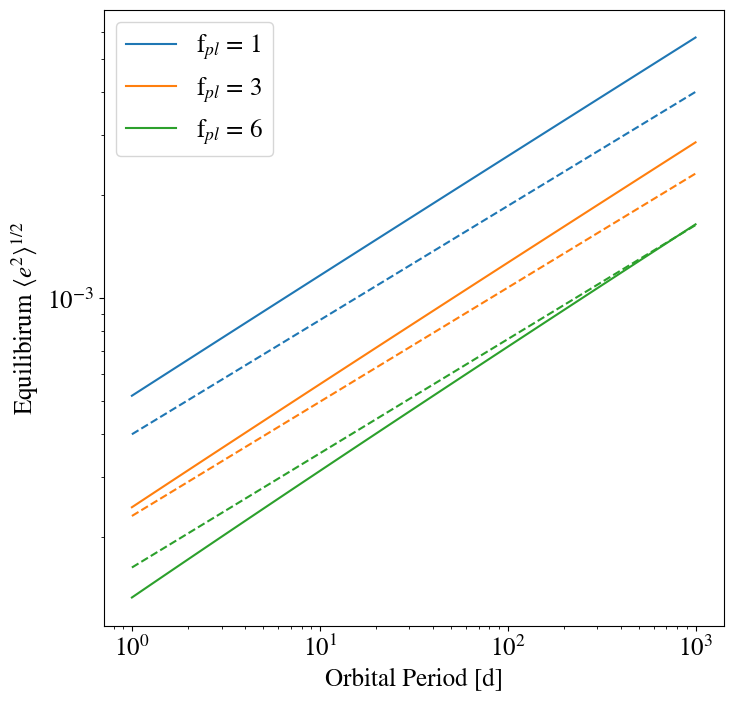
\includegraphics[width=0.5\columnwidth]{figures/time_eq_gf.png}
    \caption{Caption goes here.\label{fig:time_eq_gf}}
    \end{center}
\end{figure}

\subsection{Inhibition of Gravitational Focusing}

The scaling relations derived above assume that the collision cross section scales as $v^{-2}$ or linearly with $r$. This is only true when the planetesimal encounter velocity is small compared to the mutual escape velocity of two planetesimals. Close to the star, this condition is violated because the encounter velocity grows with the Keplerian velocity. The minimum orbital distance at which gravitational focusing is effective can be derived by equating the encounter velocity with the mutual escape velocity

\begin{equation}
    r_{gf} \geq \frac{3 M_{*} \left< e^{2} \right> s}{4 m}
\end{equation}

Another way to think of this effect is that the gravitational capture radius of a planetesimal decreases with encounter velocity. $r_{gf}$ is the orbital distance at which the capture radius is smaller than the geometric cross section of a planetesimal.  In this case, the collision timescale instead scales as 

\begin{equation}
    t_{coll} \sim A^{-1} r^{\alpha + 3/2}
\end{equation}

\noindent and the number of timesteps required to resolve a collision stays constant with $r$ for a flat ($\alpha = 0$) surface density profile.

Figure \ref{fig:time_eq_gf} also shows the minimum Hill eccentricity required to suppress gravitational focusing at a given orbital period for different values of $f_{pl}$ (dashed lines). Comparing with the solid curves, it is nearly always the case that a disk sufficiently hot enough to cause the relaxation time to exceed the collision timescale will also suppress gravitational focusing.

\subsection{Isolation Mass}

The isolation mass of a planetary embryo, which represents the largest mass that a body can attain by accreting adjacent planetesimals in the disk, is given by

\begin{equation}
    M_{iso} = 2 \pi a \left( 2 \Delta a \right) \Sigma
\end{equation}

\noindent where $a$ is the semimajor axis of the embryo and $\Delta a$ is the maximum encounter distance that results in accretion. $\Delta a$ scales with the Hill radius of the growing body, which also depends on the isolation mass.

\begin{equation}
    \Delta a = \tilde{b} R_{h} = \tilde{b} \left( \frac{M_{iso}}{3 M_{*}} \right)^{1/3} a
\end{equation}

The constant $\tilde{b}$ can be determined by requiring that adjacent protoplanets do not enter each other's Hill spheres. This is equivalent to requiring that the Jacobi energy of these bodies be negative such that \citep{Hayashi1977}

\begin{equation}
    E_{J} = \frac{1}{2} \left( \tilde{e}^{2} + \tilde{i}^{2} \right) - \frac{3}{8} \tilde{b}^{2} + \frac{9}{2}  \geq 0
\end{equation}

\noindent where $\tilde{e}$ and  $\tilde{i}$ is the eccentricity and inclination of a protoplanet in Hill units and $\tilde{b}$ is the separation between adjacent protoplanets, also in Hill units. Solving for $\tilde{b}$ gives

\begin{equation}
    \tilde{b} = \frac{2}{\sqrt{3}} \left( 9 + \tilde{e}^{2} + \tilde{i}^{2} \right)^{1/2}
\end{equation}

Finally, combining the above equations and solving for $M_{iso}$ gives

\begin{equation}
    M_{iso} = \frac{8}{\sqrt{3}} \pi^{3/2} \tilde{b}^{3/2} \Sigma^{3/2} \left( 3 M_{*} \right)^{-1/2} a^{3}
\end{equation}

Most importantly, the isolation mass depends on the eccentricities and inclinations of the planetary embryos. At large orbital periods, these quantities are damped by dynamical friction (note that this also heats the planetesimal population and makes the timescale to reach the isolation mass extremely long). At short period, however, $\tilde{e}$ and  $\tilde{i}$ can be nonzero.

\section{Summary and Discussion} \label{sec:discuss}

Summary and discussion text goes here

\bibliography{references}

\clearpage

\end{document}